%% This is file `elsarticle-template-1-num.tex',
%%
%% Copyright 2009 Elsevier Ltd
%%
%% This file is part of the 'Elsarticle Bundle'.
%% ---------------------------------------------
%%
%% It may be distributed under the conditions of the LaTeX Project Public
%% License, either version 1.2 of this license or (at your option) any
%% later version.  The latest version of this license is in
%%    http://www.latex-project.org/lppl.txt
%% and version 1.2 or later is part of all distributions of LaTeX
%% version 1999/12/01 or later.
%%
%% Template article for Elsevier's document class `elsarticle'
%% with numbered style bibliographic references
%%
%% $Id: elsarticle-template-1-num.tex 149 2009-10-08 05:01:15Z rishi $
%% $URL: http://lenova.river-valley.com/svn/elsbst/trunk/elsarticle-template-1-num.tex $
%%
\documentclass[preprint,12pt]{elsarticle}

%% Use the option review to obtain double line spacing
%% \documentclass[preprint,review,12pt]{elsarticle}

%% Use the options 1p,twocolumn; 3p; 3p,twocolumn; 5p; or 5p,twocolumn
%% for a journal layout:
%% \documentclass[final,1p,times]{elsarticle}
%% \documentclass[final,1p,times,twocolumn]{elsarticle}
%% \documentclass[final,3p,times]{elsarticle}
%% \documentclass[final,3p,times,twocolumn]{elsarticle}
%% \documentclass[final,5p,times]{elsarticle}
%% \documentclass[final,5p,times,twocolumn]{elsarticle}

%% The graphicx package provides the includegraphics command.
\usepackage{graphicx}
%% The amssymb package provides various useful mathematical symbols
\usepackage{amssymb}
%% The amsthm package provides extended theorem environments
%% \usepackage{amsthm}
\usepackage{todonotes}

%% The lineno packages adds line numbers. Start line numbering with
%% \begin{linenumbers}, end it with \end{linenumbers}. Or switch it on
%% for the whole article with \linenumbers after \end{frontmatter}.
\usepackage{lineno}

%% natbib.sty is loaded by default. However, natbib options can be
%% provided with \biboptions{...} command. Following options are
%% valid:

%%   round  -  round parentheses are used (default)
%%   square -  square brackets are used   [option]
%%   curly  -  curly braces are used      {option}
%%   angle  -  angle brackets are used    <option>
%%   semicolon  -  multiple citations separated by semi-colon
%%   colon  - same as semicolon, an earlier confusion
%%   comma  -  separated by comma
%%   numbers-  selects numerical citations
%%   super  -  numerical citations as superscripts
%%   sort   -  sorts multiple citations according to order in ref. list
%%   sort&compress   -  like sort, but also compresses numerical citations
%%   compress - compresses without sorting
%%
%% \biboptions{comma,round}

% \biboptions{}

\journal{Journal Name}

\begin{document}

\begin{frontmatter}

%% Title, authors and addresses

\title{Applying Radial Basis Function Networks and Markov Chains for on-line detection of concept drift in non-stationary environments}

%% use the tnoteref command within \title for footnotes;
%% use the tnotetext command for the associated footnote;
%% use the fnref command within \author or \address for footnotes;
%% use the fntext command for the associated footnote;
%% use the corref command within \author for corresponding author footnotes;
%% use the cortext command for the associated footnote;
%% use the ead command for the email address,
%% and the form \ead[url] for the home page:
%%
%% \title{Title\tnoteref{label1}}
%% \tnotetext[label1]{}
%% \author{Name\corref{cor1}\fnref{label2}}
%% \ead{email address}
%% \ead[url]{home page}
%% \fntext[label2]{}
%% \cortext[cor1]{}
%% \address{Address\fnref{label3}}
%% \fntext[label3]{}


%% use optional labels to link authors explicitly to addresses:
%% \author[label1,label2]{<author name>}
%% \address[label1]{<address>}
%% \address[label2]{<address>}

\author{Ruivaldo Neto}
\author{Adrien Brilhault}
\author{Ricardo Rios}

\address{Salvador, Brazil}

\begin{abstract}
The amount of data produced by computer systems has grown sharply in recent decades,
and a significant part of it is generated as uninterrupted and potentially infinite sequences known as data streams.
Generally, these streams are produced by non-stationary environments,
in which the data distribution can change over time, possibly deteriorating the system performance.
In the literature, this phenomenon is named as concept drift.
%
Nevertheless,
most concept drift detection methods are unsuited for non-stationary environments with data streams.
These algorithms usually require the correct labeling of data - infeasible in these settings -
 or do not match the strict response time and resource usage requirements.
%
This paper proposes a novel proactive on-line concept drift detection method, called RBFChain.
The proposed method relies on Radial Basis Function Networks implicit clustering property and uses Markov Chains to model the drifts transitions.
%
To assess RBFChain as a viable concept drift detector,
an analysis of sensitivity, accuracy,
and noise tolerance was performed using synthetic datasets,
and results were compared to the most established algorithms in the literature.
%
Furthermore, the technique was applied to the real-world problem of eye-tracking.
A critical issue for different areas of knowledge,
since many behavioral experiments use eye-tracking information as a relevant analysis factor.
%
Experimental results suggest that RBFChain is statistically better or equivalent to other detectors as it offers greater or equal overall classification accuracy.
Also, the method demonstrated good performance in the eye-tracking problem,
 being able to identify fixations and saccades in real-time with precision comparable to state of the art.

\end{abstract}

\begin{keyword}
Concept Drift \sep Drift Detection \sep Eye tracking
\end{keyword}

\end{frontmatter}

%%
%% Start line numbering here if you want
%%
\linenumbers

%% main text
\section{Introduction}
\label{sec:intro}
In recent years,
the volume of data produced by computer systems has grown dramatically.
Technological advances favored this growth,
such as the pervasiveness of mobile devices,
the popularization of social networks, and
the expansion of the internet of things \cite{Cohen:BigData:2009:MSN:1687553.1687576}.

A significant share of this data is produced in the form of uninterrupted and potentially infinite sequences \cite{Aggarwal:2006:DSM:1196418}.
In the literature,
sequences with these characteristics are known as data streams.
These streams are present in various fields of application,
such as financial market monitoring  \cite{ZHOU:2015},
road traffic monitoring \cite{Wang:2015:EOV:2843092.2843464},
telecom network management \cite{delattre2015method},
real-time sentiment analysis  \cite{KRANJC2015187}
and intruder prevention and identification systems \cite{KENKRE:PAI:COLACO:2015}.

Most of the environments that produce data streams are non-stationary.
That is,
the joint probability distribution changes arbitrarily over time,
such as a switch in the conditional probability distribution on a classification problem,
or a change of some moment (such as mean and variance) on a time series forecasting problem \cite{tsymbal2004problem}.
Systems applied to these environments may be unable to adapt to the new information, hence dramatically deteriorating their performance.
This phenomenon is known as concept drift \cite{Gama:2014:DAF:2670967.2670971}.
%
Still, most concept drift detection methods are inapplicable in those environments.
These methods usually require the correct labeling of data - impracticable in those contexts -
 or do not meet the severe response time and resource usage restrictions inherent to scenarios with data streams.

This paper proposes a novel proactive on-line concept drift detection method, called RBFChain.
The proposed algorithm is based on Radial Basis Function Networks implicit clustering property
and employs Markov Chains to model the drifts transitions.
To validate the proposed method as a viable concept drift detector,
an examination of sensitivity, accuracy,
and noise tolerance was performed using synthetic datasets,
and results were compared to the most established algorithms in the literature.
%
Moreover, the algorithm was also applied to the real-world problem of eye-tracking.
A problem with impact in different areas of knowledge, since many behavioral experiments use eye-tracking information as a relevant analysis factor.

Experimental results suggest that RBFChain is statistically better or equivalent to other detectors as it offers greater or equal overall classification accuracy.
Additionally, the method demonstrated good performance in the eye-tracking problem,
being able to identify fixations and saccades in real-time with precision comparable to state of the art.

The rest of the paper is organized as follows:
Section 2 describes the concept drift phenomenon and the main detection techniques;
Section 3 presents the eye-tracking problem;
Section 4 describes the RBFChain algorithm and its pseudo-code;
Section 5 presents the setup and results of the experiment with synthetic datasets;
Section 6 shows the setup and results of the eye-tracking experiment;
and, finally, Section 7 provides conclusions and discusses future work.

\section{Concept Drift}
\label{sec:concept_drift}

Most real-world problems scenarios can be regarded as non-stationary environments \cite{Gama:2014:DAF:2670967.2670971}.
In these environments, the joint probability distribution can change over time,
such as a switch in the conditional probability distribution on a classification problem,
or a change of some moment (such as mean and variance) on a time series forecasting problem \cite{tsymbal2004problem}.
%
Systems applied to these settings may be unable to adapt to the changes, hence dramatically deteriorating their performance.
This phenomenon is known as concept drift.

The Bayesian Theory can be used to formally define the concept drift phenomenon \cite{Elwell:2011}:
consider the posterior probability of a sample $x$ belonging to a class $y$, a concept drift happens when this probability changes over time, that is, $Pt + 1 (y | x) \neq Pt (y | x)$. In a supervised learning scenario, this can be interpreted as when the relationship between the input data and the target variable change over time.

According to \cite{tsymbal2004problem, Gama:2014:DAF:2670967.2670971}, concept drifts can occur in four main patterns.
These patterns are demonstrated in Figure \ref{fig:concept_drift_patterns} and described below:

\begin{itemize}
    \item \textbf{Abrupt:} occurs when a concept A switches abruptly to another concept B.
    \item \textbf{Gradual:} occurs when a concept A is being exchanged for the B concept slowly. In this case, while there is no definitive change from concept A to concept B, occurrences of B become more frequent, while fewer events of A are observed.
    \item \textbf{Incremental:} occurs when a concept A is being exchanged for B through intermediate concepts.  These concepts differ little from its predecessor and successor, so changes are noticeable only in the long run.
    \item \textbf{Recurrent:} occurs when a previously active concept reappears after a certain period. However, this cannot be understood as a periodic seasonality.
\end{itemize}

\begin{figure}[h!]
\begin{center}
    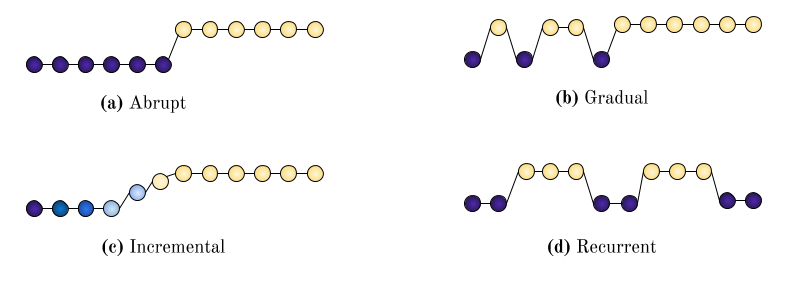
\includegraphics[scale=0.7]{img/concept_drift_patterns.png}
    \caption{Concept Drift Patterns}
    \label{fig:concept_drift_patterns}
\end{center}
\end{figure}

Concept drift detection methods characterize and quantify concept drifts through the delimitation of moments or time intervals in which change happens \cite{Basseville:1993:DAC:151741}.
%
These algorithms fall into two categories, according to the need for data labeling \cite{Zliobaite:2010}:

\begin{itemize}
    \item \textbf{Explicit Algorithms/Supervised}: Adopt a reactive approach, as they depend on the correct labeling of the data.
    The model performance is monitored continuously, and drifts are detected when its performance starts to deteriorate, passing past a threshold.
    \item \textbf{Implicit Algorithms/Unsupervised:} Implement a proactive approach and are independent of data labels.
    Concept drifts are detected through the analysis of incoming data or indicators produced by the applied learning techniques.
    Although more prone to false alarms, they are an alternative to scenarios where obtaining labels is expensive, time-consuming, or unviable.
    Also, this approach can lead to better results, since it is possible to refit the model or adjust the data before the deterioration of the predictions.
\end{itemize}

This paper proposes a novel unsupervised and proactive concept drift detection method.
The algorithm continually groups the incoming data through Radial Basis Function Networks and maintains a model of the center transitions in a Markov Chain.
Drifts are detected when the probability of a transition in the formed cluster reaches a parametric threshold.

\section{Eye-tracking}
\label{sec:eye_tracking}

\ldots

\section{RBFChain algorithm}
\label{sec:rbfchain_algorithm}

This section details the RBFChain implementation. However, before describing the proposed method, it is significant to present the main applied concepts of Radial Base Function Networks and Markov Chains.

\subsection{Radial Basis Function Networks (RBFN)}

Radial Basis Function Networks (RBFN) are used in various disciplines with a reasonable degree of success. The broad applicability is a result of their excellent ability to make function approximation, especially when the relationships among the variables of interest are nonlinear \cite{Bishop:2006:PRM:1162264}.

A radial basis function network is a type of artificial neural network (ANN), and most neural networks are known to be useful in modeling complex and nonlinear relationships. An RBFN has advantages in specific applications in that for a given parameter set, RBFN networks do not require an iterative procedure to learn the model. Iterative learning for most ANN types is computationally expensive and vulnerable to the local minima problem.

The topology of an RBFN is given in Fig. \ref{fig:rbg_arq} as a multiple input single output feedforward network.
Assume that there are $n$ input variables labeled from $x_1$ to $x_n$.
The network receives input samples as vectors $x=(x_1, x_2, \ldots, x_n)$ of size $1 \times n$.
The initial layer is only a buffer that feeds the input values to the intermediate layer, which is called the hidden layer.
There are $n_h$ processing elements in the hidden layer.
Each processing element in the hidden layer processes the input vector and produces a single value output. This processing is performed through a basis function $\phi$.
Finally, the output layer weights the results of the intermediate layer by weights, aggregating them linearly to compose the final network response.

Among many candidates for basis functions, Gaussian radial basis function (RBF), presented in Eq. \ref{eq:gaussian}, is used in this study. The main reason for this choice is that it can be shown that an RBFN with Gaussian RBF can sufficiently approximate any given function for a large enough number of hidden layer elements \cite{Theodoridis:2008:PRF:1457541}.

Probabilistic methods are built on soft decision rules, which are formalized as probabilities, e.g.,  the probability of a data point being a saccade given the previous observations. The probabilities – and thus, the decisions – are adjusted to the observations.


\begin{equation}
    \label{eq:gaussian}
    \varphi (v_{i})=e^{-(\sigma r)^{2}}
\end{equation}

In the hidden layer, each processing element has a separate vector called the center, which has the same dimensions as the input vector.
For $n_h$ hidden layer elements we have $n_h$ center vectors as $(c_1; c_2; \ldots; {c_n}_h)$.
Then each processing element looks at the distance between the input vector and its center and uses this distance to create its output (activation phase).


This work uses only the initial and intermediary layers of the presented architecture.
The initial layer channels the incoming data to the middle layer, which implicitly forms clusters during the activation phase.
The formed grouping has an active center that changes according to the processed value.
Changes in the active center are interpreted as possible concept drifts.

\begin{figure}[h!]
\begin{center}
    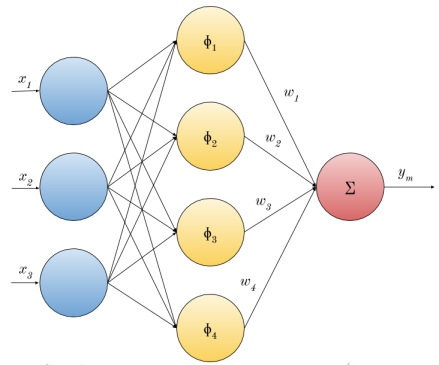
\includegraphics[scale=0.75]{img/rbf_arq.png}
    \caption{Topology of a RBFN}
    \label{fig:rbg_arq}
\end{center}
\end{figure}


\subsection{Markov Chains}

A Markov chain model can be defined by the tuple $(S; A; \lambda)$. S corresponds to the state space, A is a matrix representing transition probabilities from one state to another, and $\lambda$ is the initial probability distribution of the states in S. If there are $n$ states in our Markov chain, then the
matrix of transition probabilities $A$ is of size $n \times n$.

The fundamental property of the Markov model is the dependency on the previous state. If the vector $s(t)$ denotes the probability vector for all the states at time $t$, then:

\begin{equation}
    \label{eq:markov}
    \hat { s } ( t ) = \hat { s } ( t - 1 ) A
\end{equation}

In this proposal, Markov chains are used to model the transitions (activations) between centers in the Radial Basis Function Network.
For this formulation, a Markov state corresponds to one of the centers.

When the RBFN identifies a different center, a new state is registered in the Markov Chain.
Initially, all possible transitions from this center have a zero value.
If another center is activated, this change produces an increment in the probability of the correspondent transition.
In paralell, all other transitions probabilites are decreased proportionally to the total number of possible transitions.

The use of a Markov Chain allows the proposed algorithm to keep an online model of the transitions. The probabilities sustained in this model are compared to parametric thresholds, to indicate when a warning zone is triggered, or a concept drift happens.

\subsection{RBFChain}

\ldots

\section{Analyses on Synthetic Datasets with Concept Drift}
\label{sec:results_synthetic_dataset}

\subsection{Experimental Setup}

\subsection{Results}

\section{Detection of Saccade and Fixation}
\label{sec:detection_of_saccade_and_fixation}

\subsection{Experimental Setup}

\subsection{Results}

\section{Concluding Remarks}

\bibliographystyle{model1-num-names}
\bibliography{references}

\end{document}

%%
%% End of file `elsarticle-template-1-num.tex'.